\documentclass[letterpaper,12pt,fleqn]{article}
\usepackage{matharticle}
\usepackage{graphtheory}
\pagestyle{empty}
\begin{document}

\section*{Common Graph Classes}

\begin{enumerate}[left=0pt]

\item Empty \((E_n)\)
  \begin{gather*}
    V(E_n)=\set{1,\ldots,n} \\
    E(E_n)=\emptyset \\
    \abs{V(E_n)}=n \\
    \abs{E(E_n)}=0 \\
    E_n\ \text{is connected}\ \iff n=1
  \end{gather*}

  \begin{examples}
    \begin{minipage}{1.5in}
      \begin{center}
        \begin{tikzpicture}[every node/.style=unlabeled node]
          \node at (0,0) {};
        \end{tikzpicture}

        \bigskip

        \(E_1\)
      \end{center}
    \end{minipage}
    \begin{minipage}{2.5in}
      \begin{center}
        \begin{tikzpicture}[every node/.style=unlabeled node]
          \pathNnodes{4}{(0,0)}{right}{};
        \end{tikzpicture}

        \bigskip

        \(E_4\)
      \end{center}
    \end{minipage}
    \begin{minipage}{2in}
      \begin{center}
        \begin{tikzpicture}[every node/.style=unlabeled node]
          \pathNnodes{3}{(0,0)}{right}{};
          \pathNnodes{3}{(0,1)}{right}{};
          \pathNnodes{3}{(0,2)}{right}{};
        \end{tikzpicture}

        \bigskip

        \(E_9\)
      \end{center}
    \end{minipage}
  \end{examples}

  The null graph is represented by \(E_0\).

  \bigskip

\item Path \((P_n)\)
  \begin{gather*}
    V(P_n)=\set{1,\ldots,n} \\
    E(P_n)=\set{\set{1,2},\set{2,3},\ldots,\set{n-1,n}} \\
    \abs{V(P_n)}=n \\
    \abs{E(P_n)}=n-1 \\
    P_n\ \text{is connected} \\
    \diam(P_n)=n-1
  \end{gather*}

  \begin{examples}
    \begin{minipage}{1.5in}
      \begin{center}
        \begin{tikzpicture}[every node/.style=unlabeled node]
          \node at (0,0) {};
        \end{tikzpicture}

        \bigskip

        \(P_1\)
      \end{center}
    \end{minipage}
    \begin{minipage}{2.5in}
      \begin{center}
        \begin{tikzpicture}[every node/.style=unlabeled node]
          \pathN{4}{(0,0)}{right}{};
        \end{tikzpicture}

        \bigskip

        \(P_4\)
      \end{center}
    \end{minipage}
    \begin{minipage}{2in}
      \begin{center}
        \begin{tikzpicture}[every node/.style=unlabeled node]
          \pathNnodes{3}{(0,0)}{right}{b};
          \pathNnodes{3}{(0,1)}{right}{m};
          \pathNnodes{3}{(0,2)}{right}{t};
          \draw (t1) to (t2) to (t3) to (m3) to (m2) to (m1) to (b1) to (b2) to (b3);
        \end{tikzpicture}

        \bigskip

        \(P_9\)
      \end{center}
    \end{minipage}
  \end{examples}

  \bigskip

\item Cycle \((C_n)\)
  \begin{gather*}
    V(C_n)=\set{1,\ldots,n} \\
    E(C_n)=\set{\set{1,2},\set{2,3},\ldots,\set{n-1,n},\set{n,1}} \\
    \abs{V(C_n)}=n\ge 3 \\
    \abs{E(C_n)}=n\ge 3 \\
    C_n\ \text{is connected} \\
    \diam(P_n)=\floor*{\frac{n}{2}}
  \end{gather*}

  \begin{examples}
    \begin{minipage}{2in}
      \begin{center}
        \begin{tikzpicture}[every node/.style=unlabeled node]
          \cycleN{3}{(0,0)}{0.5in}{90}{};
        \end{tikzpicture}

        \bigskip

        \(C_3\)
      \end{center}
    \end{minipage}
    \begin{minipage}{2in}
      \begin{center}
        \begin{tikzpicture}[every node/.style=unlabeled node]
          \cycleN{4}{(0,0)}{0.5in}{135}{};
        \end{tikzpicture}

        \bigskip

        \(C_4\)
      \end{center}
    \end{minipage}
    \begin{minipage}{2in}
      \begin{center}
        \begin{tikzpicture}[every node/.style=unlabeled node]
          \cycleN{9}{(0,0)}{0.5in}{90}{};
        \end{tikzpicture}

        \bigskip

        \(C_9\)
      \end{center}
    \end{minipage}
  \end{examples}

  \bigskip

\item Complete \((K_n)\)
  \begin{gather*}
    V(K_n)=\set{1,\ldots,n} \\
    E(K_n)=\ps_2\left(V(K_n)\right) \\
    \abs{V(K_n)}=n \\
    \abs{E(K_n)}=\binom{n}{2}=\frac{n(n-1)}{2} \\
    K_n\ \text{is connected} \\
    \diam(P_n)=1\iff G=K_n
  \end{gather*}

  \begin{examples}
    \begin{minipage}{2in}
      \begin{center}
        \begin{tikzpicture}[every node/.style=unlabeled node]
          \node at (0,0) {};
        \end{tikzpicture}

        \bigskip

        \(K_1\)
      \end{center}
    \end{minipage}
    \begin{minipage}{2in}
      \begin{center}
        \begin{tikzpicture}[every node/.style=unlabeled node]
          \completeN{4}{(0,0)}{0.5in}{135}{};
        \end{tikzpicture}

        \bigskip

        \(K_4\)
      \end{center}
    \end{minipage}
    \begin{minipage}{2in}
      \begin{center}
        \begin{tikzpicture}[every node/.style=unlabeled node]
          \completeN{9}{(0,0)}{0.5in}{90}{};
        \end{tikzpicture}

        \bigskip

        \(K_9\)
      \end{center}
    \end{minipage}
  \end{examples}

\item Petersen Graph (PG)
  \begin{gather*}
    \abs{V(PG)}=10 \\
    \abs{E(PG)}=10 \\
    PG\ \text{is connected}
  \end{gather*}

  The vertices represents the \(2\)-subsets of a \(5\) element set and the edges indicate disjoint sets.

  \begin{center}
    \begin{tikzpicture}[every node/.style={labeled node}]
      \cycleV{\(\set{a,b}\),\(\set{d,e}\),\(\set{a,c}\),\(\set{b,e}\),\(\set{c,d}\)}{(0,0)}{2in}{90}{o};
      \cycleVnodes{\(\set{c,e}\),\(\set{b,c}\),\(\set{b,d}\),\(\set{a,d}\),\(\set{a,e}\)}{(0,0)}{1in}{90}{i};
      \draw (i1) to (i3) to (i5) to (i2) to (i4) to (i1);
      \foreach \i in {1,2,3,4,5}{
        \draw (o\i) to (i\i);
      }
    \end{tikzpicture}
  \end{center}

\item Cube Graph (\(Q_n\))
  \begin{gather*}
    \abs{V(PG)}=2^n \\
    \abs{E(PG)}=n2^n \\
    Q_n\ \text{is connected}
  \end{gather*}

  The vertices represents the bit strings of length \(n\) and the edges indicate a one bit difference.

  \begin{examples}
    \begin{minipage}{1in}
      \begin{center}
        \scalebox{0.75}{
            \begin{tikzpicture}[every node/.style=labeled node]
              \node at (0,0) {\(0\)};
            \end{tikzpicture}
        }

        \bigskip

        \(Q_0\)
      \end{center}
    \end{minipage}
    \begin{minipage}{1.25in}
      \begin{center}
        \scalebox{0.75}{
          \begin{tikzpicture}[every node/.style=labeled node,node distance=1in]
            \pathV{\(0\),\(1\)}{(0,0)}{right}{}
          \end{tikzpicture}
        }

        \bigskip

        \(Q_1\)
      \end{center}
    \end{minipage}
    \begin{minipage}{1.25in}
      \begin{center}
        \scalebox{0.75}{
          \begin{tikzpicture}[every node/.style=labeled node]
            \cycleV{\(00\),\(01\),\(11\),\(10\)}{(0,0)}{0.5in}{135}{o};
          \end{tikzpicture}
        }

        \bigskip

        \(Q_2\)
      \end{center}
    \end{minipage}
    \begin{minipage}{2.5in}
      \begin{center}
        \scalebox{0.75}{
          \begin{tikzpicture}[every node/.style=labeled node]
            \cycleV{\(100\),\(101\),\(111\),\(110\)}{(0,0)}{1.5in}{135}{o};
            \cycleV{\(000\),\(001\),\(011\),\(010\)}{(0,0)}{0.75in}{135}{i};
            \foreach \i in {1,2,3,4}{
              \draw (o\i) edge (i\i);
            }
          \end{tikzpicture}
        }

        \bigskip

        \(Q_3\)
      \end{center}
    \end{minipage}

    \bigskip
    
    \begin{center}
      \scalebox{0.75}{
        \begin{tikzpicture}[every node/.style=labeled node]
          \cycleV{\(1000\),\(1001\),\(1011\),\(1010\),\(1110\),\(1111\),\(1101\),\(1100\)}{(0,0)}{3.5in}{90}{o};
          \cycleV{\(0000\),\(0001\),\(0011\),\(0010\),\(0110\),\(0111\),\(0101\),\(0100\)}{(0,0)}{1in}{90}{i};
          \foreach \i in {1,2,...,8}{
            \draw (o\i) edge (i\i);
          }
          \draw (i1) edge (i4);
          \draw (i2) edge (i7);
          \draw (i3) edge (i6);
          \draw (i5) edge (i8);
          \draw (o1) edge (o4);
          \draw (o2) edge (o7);
          \draw (o3) edge (o6);
          \draw (o5) edge (o8);
        \end{tikzpicture}
      }
      
      \bigskip

      \(Q_4\)
    \end{center}
  \end{examples}

\end{enumerate}

\end{document}
